\subsection{マップ・詳細画面}
マップ・詳細画面は、ツールバー、マップ、カードから構成されている。ツールバーはカードリスト画面へ戻るために画面上部に表示している。マップはユーザの現在地や観光スポットの場所を見るために画面中央に表示している。カードは観光スポットの場所とそこに関する情報を関連づけて見ることを可能とするために、観光スポットのタイトルと写真および紹介文を画面下部に表示している。\\
本画面へ遷移してきた際の初期動作は、カードリスト画面でユーザがタップしたカードに対応する観光スポットの場所をピンとしてマップ中央に表示することである。また、カードリスト画面でユーザがお気に入りとして星をつけた場合は対応する観光スポットの場所を星としてマップ上に表示する。マップ上に表示しているピンまたは星をタップすることで、画面下部のカードに記載している情報が対応する観光スポットの情報へと切り替わる仕様である。初期状態では、画面下部のカードの情報はお店の営業時間や有名商品の値段などを表示(図6.2(a))しているが、右向きの矢印をタップすることでカードリスト画面にも表示している観光スポットの紹介文へと表示内容が切り替わる(図6.2(b))。観光スポットの紹介文を表示している間は左向きの矢印となり、それをタップすることで初期状態の詳細情報の表示へと切り替わる。マップ・詳細画面で使用したアイコンの意味については表6.2を参照されたい。

\begin{table}[htb]
\centering
\addtocounter{table}{+0}
\caption{アイコン一覧と意味}
  \begin{tabular}{|c|c|} \hline
    アイコン&意味  \\ \hline 
    \begin{minipage}{10mm}
      \centering
      \scalebox{0.4}{
\includegraphics{redpin.png}}
    \end{minipage} & \parbox{38zw}{本画面への画面遷移直前にタップした観光スポットの場所を示すピン。} \\  \hline
    \begin{minipage}{10mm}
      \centering
      \scalebox{0.3}{
\includegraphics{favourites.png}}
    \end{minipage} &\parbox{38zw}{カードリスト画面で星ボタンを押したカードの観光スポットの場所を示すピン。}\\ \hline
     \begin{minipage}{10mm}
      \centering
      \scalebox{0.5}{
\includegraphics{arrow.png}}
    \end{minipage} & \parbox{38zw}{観光スポットの詳細情報と紹介文の表示を切り替えるためのボタン。}\\ \hline
  \end{tabular} 
\end{table}

\newpage

\begin{figure}[htbp]
  \begin{center}
    \begin{tabular}{c}

      % 1
      \begin{minipage}{0.33\hsize}
        \begin{center}
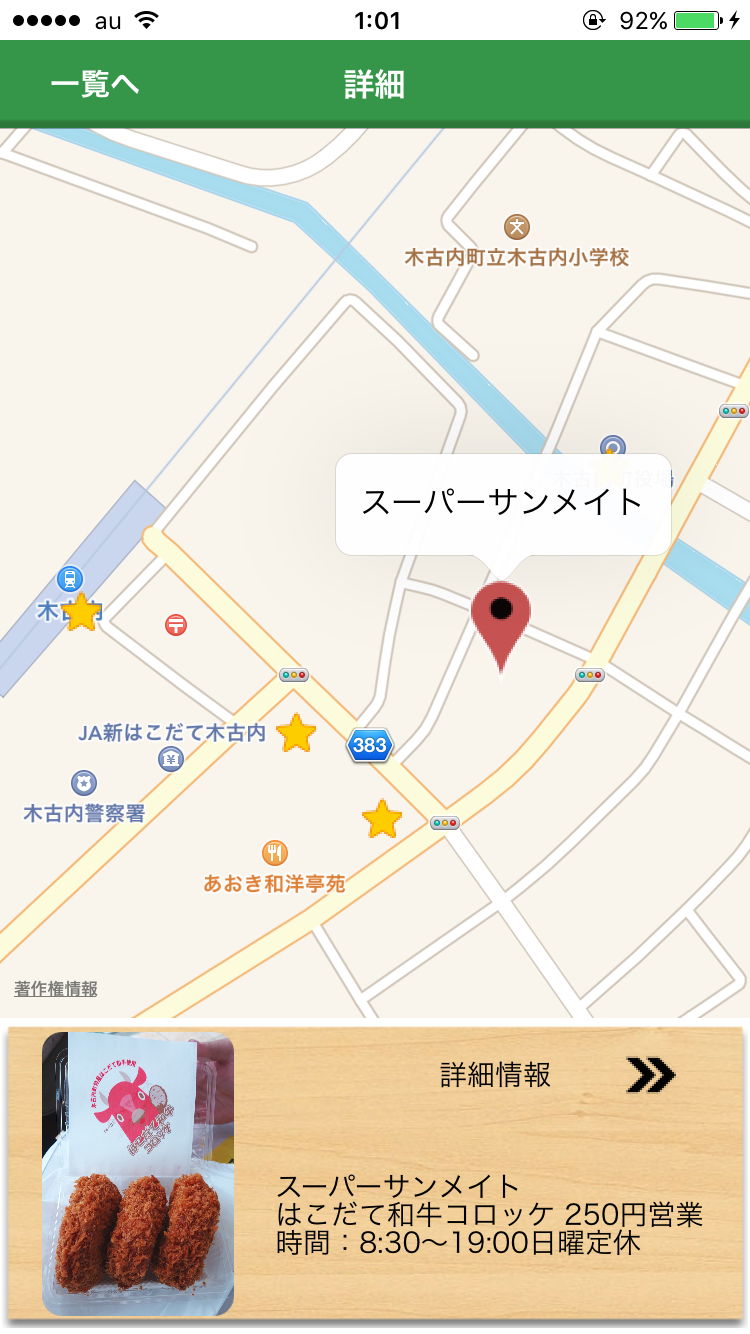
\includegraphics[width=4cm, bb=0 0 705 1334]{kiko_map1.png}
         \hspace{1cm} %(a)観光スポットの詳細情報を表示中
          {\footnotesize (a)観光スポットの詳細情報を表示中}
        \end{center}
      \end{minipage}

      % 2
      \begin{minipage}{0.33\hsize}
        \begin{center}
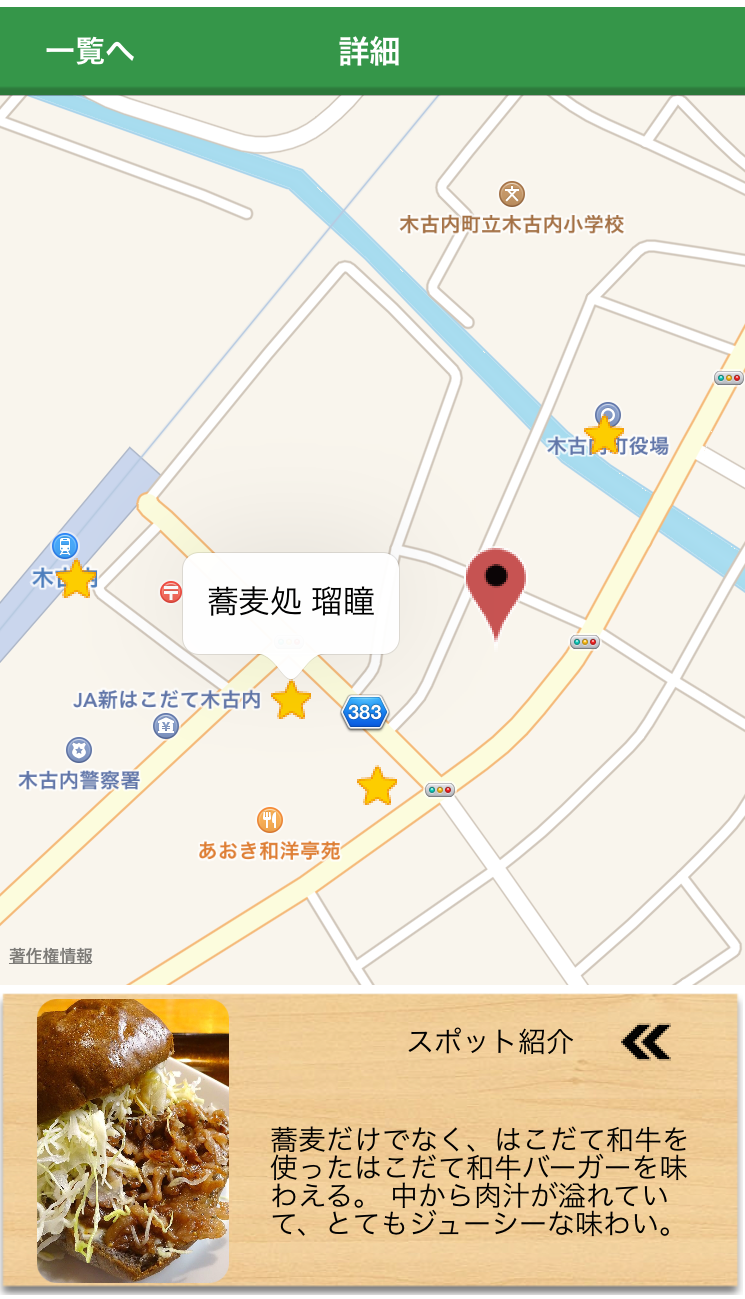
\includegraphics[width=4cm, bb=0 0 705 1334]{kiko_map2.png}
          \hspace{1cm} %(b)観光スポットの紹介文を表示中
          {\footnotesize (b)観光スポットの紹介文を表示中}
        \end{center}
      \end{minipage}

    \end{tabular}
    \caption{マップ・詳細画面}
    \label{fig:lena}
  \end{center}
\end{figure}
\
\bunseki{岩見建汰}